\section{Publishing \& approval}
\label{sec:settings-feature-publishing-approval}

This page decides which changes someone else must review before they reach members, so daily work is not hurt by a hasty edit. It has three independent tabs, each with its own policy and Save button: “Forms”, “Record types” and “Procedure cards”. The policy stays off until you turn it on. The page appears for the organization owner and holders of the Administrator role; what others see differs by tab.

\begin{rcnote}[Example: Horizon]
The system administrator chooses “For all forms” at ①, writes a stage called “HR review” at ②, names Sarah Al-Khatib as reviewer, then presses “Save” at ⑤. If Omar Haddad changes the visit request form, the new version is not published until Sarah approves it.
\end{rcnote}

\begin{figure}[H]
\centering
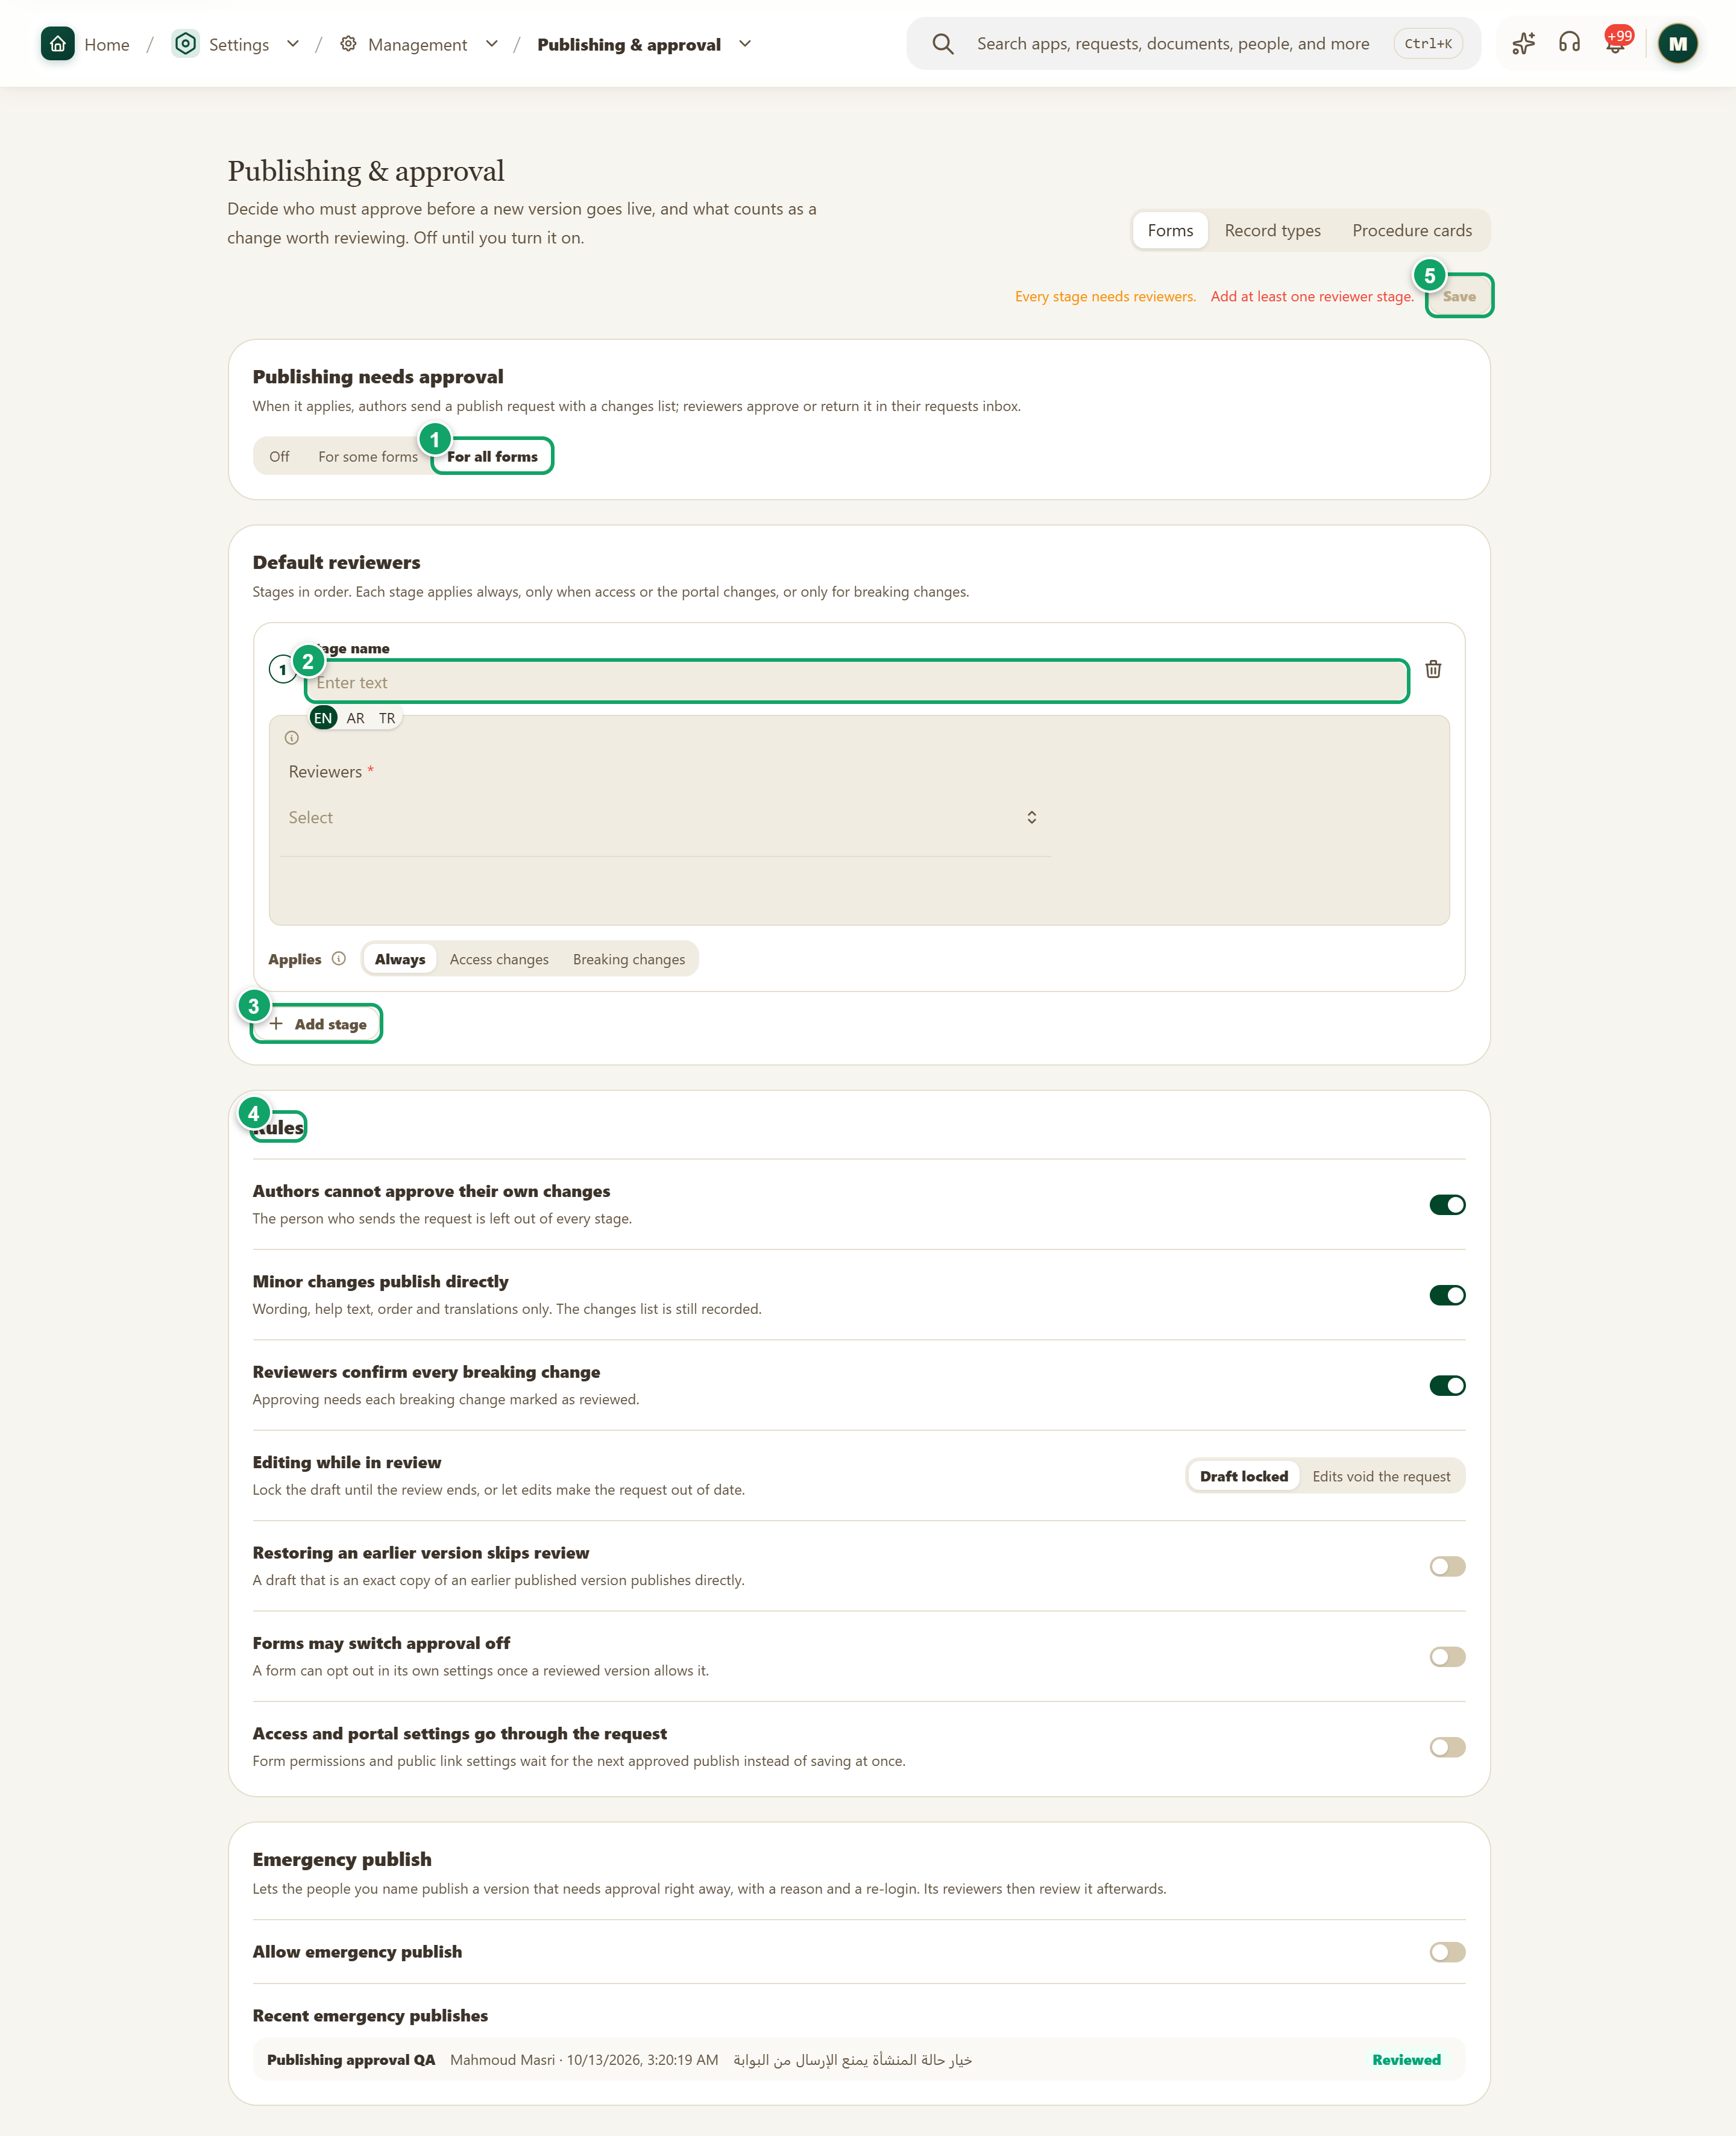
\includegraphics[width=0.95\linewidth,height=0.72\textheight,keepaspectratio]{figures/screens/ch08-publishing-approval-en.png}
\caption{The publishing policy on the Forms tab}
\label{fig:settings-publishing-approval-screen}
\shotnote{The image shows a trial edit that was not saved: “For all forms” is chosen and an empty stage added, so two warnings appear and Save stays disabled. The policy cannot be saved until you say who reviews. “Recent emergency publishes” shows an entry from test data. ① “For all forms”: the policy’s scope. ② “Stage name”. ③ “Add stage”. ④ “Rules”. ⑤ “Save”.}
\end{figure}

\begin{table}[H]
\centering
\caption{What do you record on the Forms tab?}
\label{tab:settings-publishing-approval-forms}
\begin{tabularx}{\linewidth}{R{4.2cm} Y}
\rcHeaderRow
\thh{Setting} & \thh{What does it decide?}\\
“Publishing needs approval” & “Off”, “For some forms” or “For all forms”.\\
“Forms covered” & Appears with “For some forms”: “Offered on the public portal or through a service”, “With approval steps” and “That write to records”.\\
“Default reviewers” & Stages in order, up to 6. Each has “Stage name”, “Reviewers” and “Applies”: “Always”, “Access changes” or “Breaking changes”.\\
“Authors cannot approve their own changes” & The person who sends the request is left out of every stage.\\
“Minor changes publish directly” & Wording, help text, order and translations need no review, and stay recorded in the changes list.\\
“Reviewers confirm every breaking change” & A breaking change removes a question or option, changes a question’s type, or changes how answers are written to records. The reviewer must mark each one “Reviewed”.\\
“Editing while in review” & “Draft locked” until the review ends, or “Edits void the request”.\\
“Restoring an earlier version skips review” & A draft that is an exact copy of an earlier published version publishes directly.\\
“Forms may switch approval off” & A form can opt out in its own settings once a reviewed version allows it.\\
“Access and portal settings go through the request” & Form permissions and public link settings wait for the next approved publish instead of saving at once.\\
“Emergency publish” & When on, you set “Who may publish in an emergency” and “Post-review within”, from 1 to 14 days. They publish at once with a reason and a re-login, and reviewers review the version afterwards.\\
\end{tabularx}
\end{table}

\begin{figure}[H]
\centering
\begin{tikzpicture}[node distance=0.5cm]
\node[stepBox] (a) {The designer writes the draft};
\node[stepBox,below=of a] (b) {They send a publish request with a changes list};
\node[stepBox,below=of b] (c) {Reviewers review it stage by stage};
\node[stepBox,below=of c] (d) {The version goes live once approved};
\draw[flowsTo] (a) -- (b);
\draw[flowsTo] (b) -- (c);
\draw[flowsTo] (c) -- (d);
\end{tikzpicture}
\rclegend
\caption{A form version’s path with the policy on}
\label{fig:settings-publishing-approval-flow}
\shotnote{The diagram shows what changes for form designers once the policy is on: publishing becomes a request that reaches reviewers in “Requests for you”, where they approve or return it. The current version stays in use meanwhile, so tell your designers before turning it on.}
\end{figure}

\begin{figure}[H]
\centering
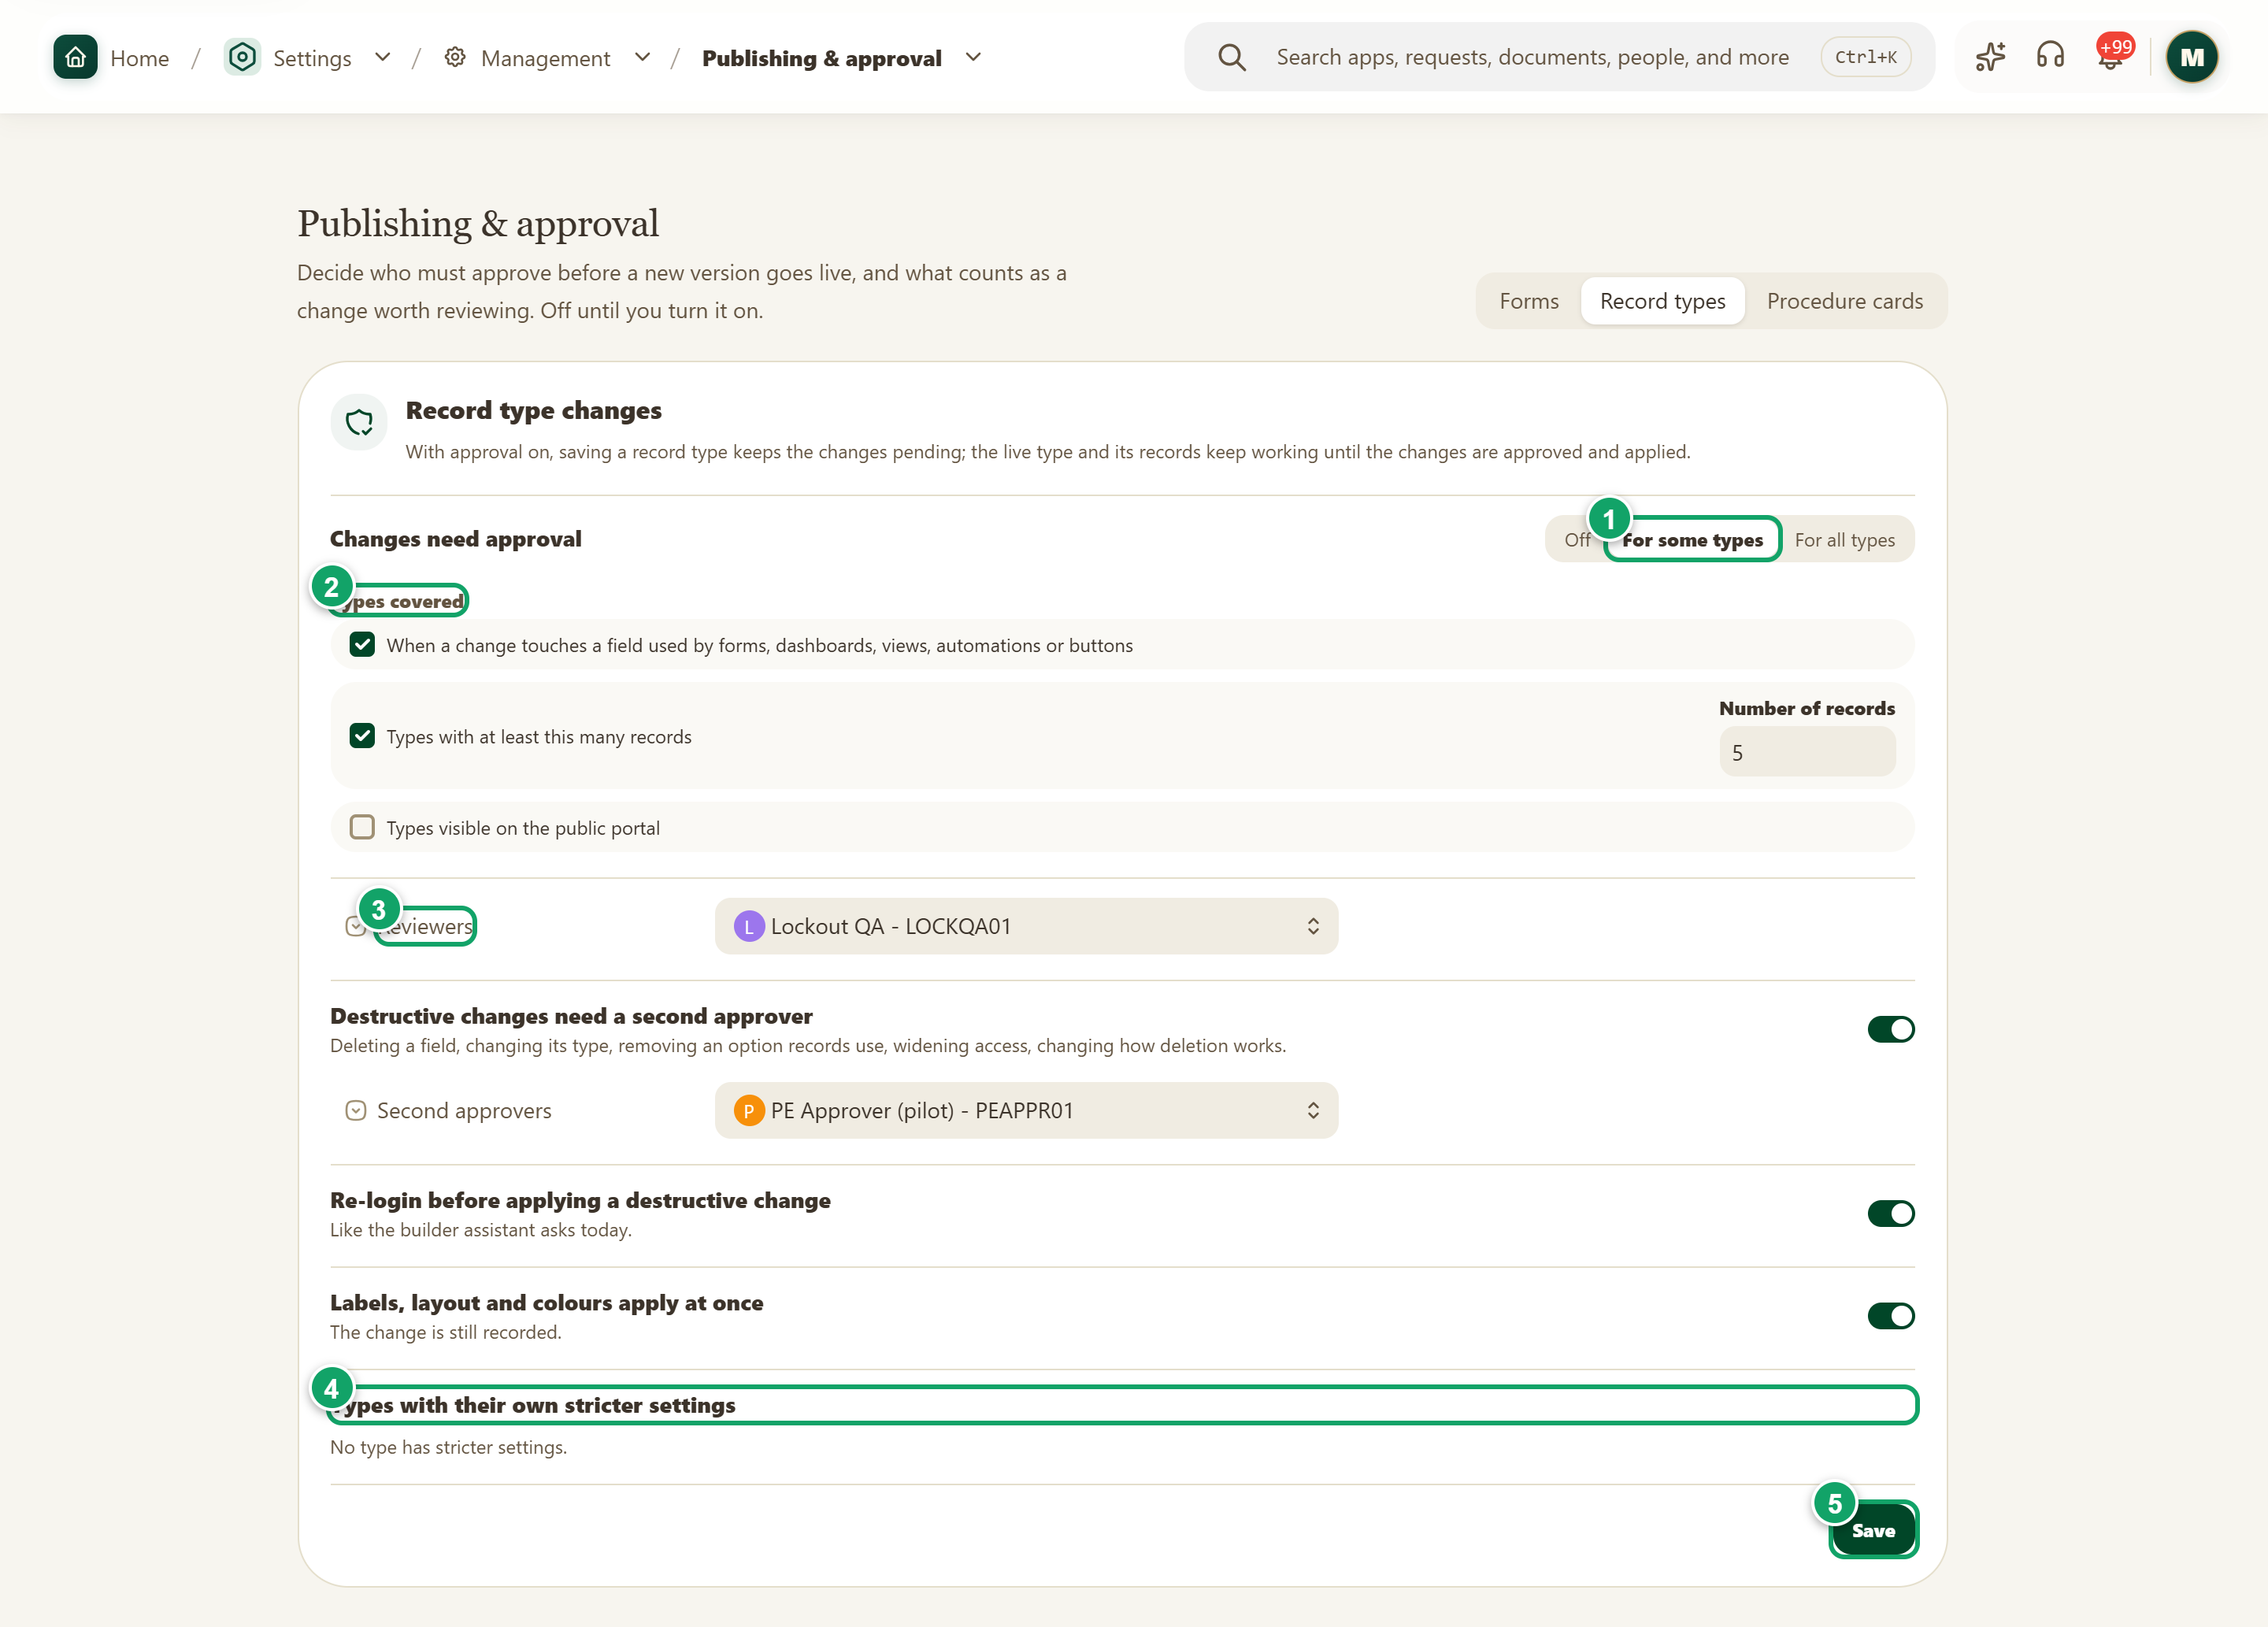
\includegraphics[width=0.95\linewidth,height=0.72\textheight,keepaspectratio]{figures/screens/ch08-publishing-approval-record-types-en.png}
\caption{The policy on the Record types tab}
\label{fig:settings-publishing-approval-record-types-screen}
\shotnote{The image shows “For some types” chosen without saving, which reveals the hidden fields; the test organization’s saved policy is off. With the policy on, the current type and its records keep working until pending changes are approved and applied. ① “For some types”. ② “Types covered”. ③ “Reviewers”: one approval is enough, and the author’s own approval does not count. ④ “Types with their own stricter settings”. ⑤ “Save”.}
\end{figure}

\begin{table}[H]
\centering
\caption{What do you record on the Record types tab?}
\label{tab:settings-publishing-approval-record-types}
\begin{tabularx}{\linewidth}{R{4.2cm} Y}
\rcHeaderRow
\thh{Setting} & \thh{What does it decide?}\\
“Changes need approval” & “Off”, “For some types” or “For all types”.\\
“Types covered” & A change touching a field used by forms, dashboards, views, automations or buttons; types that reached the set “Number of records”; or types shown on the public portal.\\
“Destructive changes need a second approver” & Deleting a field, changing its type, deleting an option records use, widening permissions, or changing the delete mode. You also set the “Second approvers”.\\
“Re-login before applying a destructive change” & The person signs in again before applying.\\
“Labels, layout and colours apply at once” & These changes do not wait for approval, and the change stays recorded.\\
“Types with their own stricter settings” & The types with their own rules, stricter than the general policy; “Remove” deletes a type’s own rule.\\
\end{tabularx}
\end{table}

\begin{figure}[H]
\centering
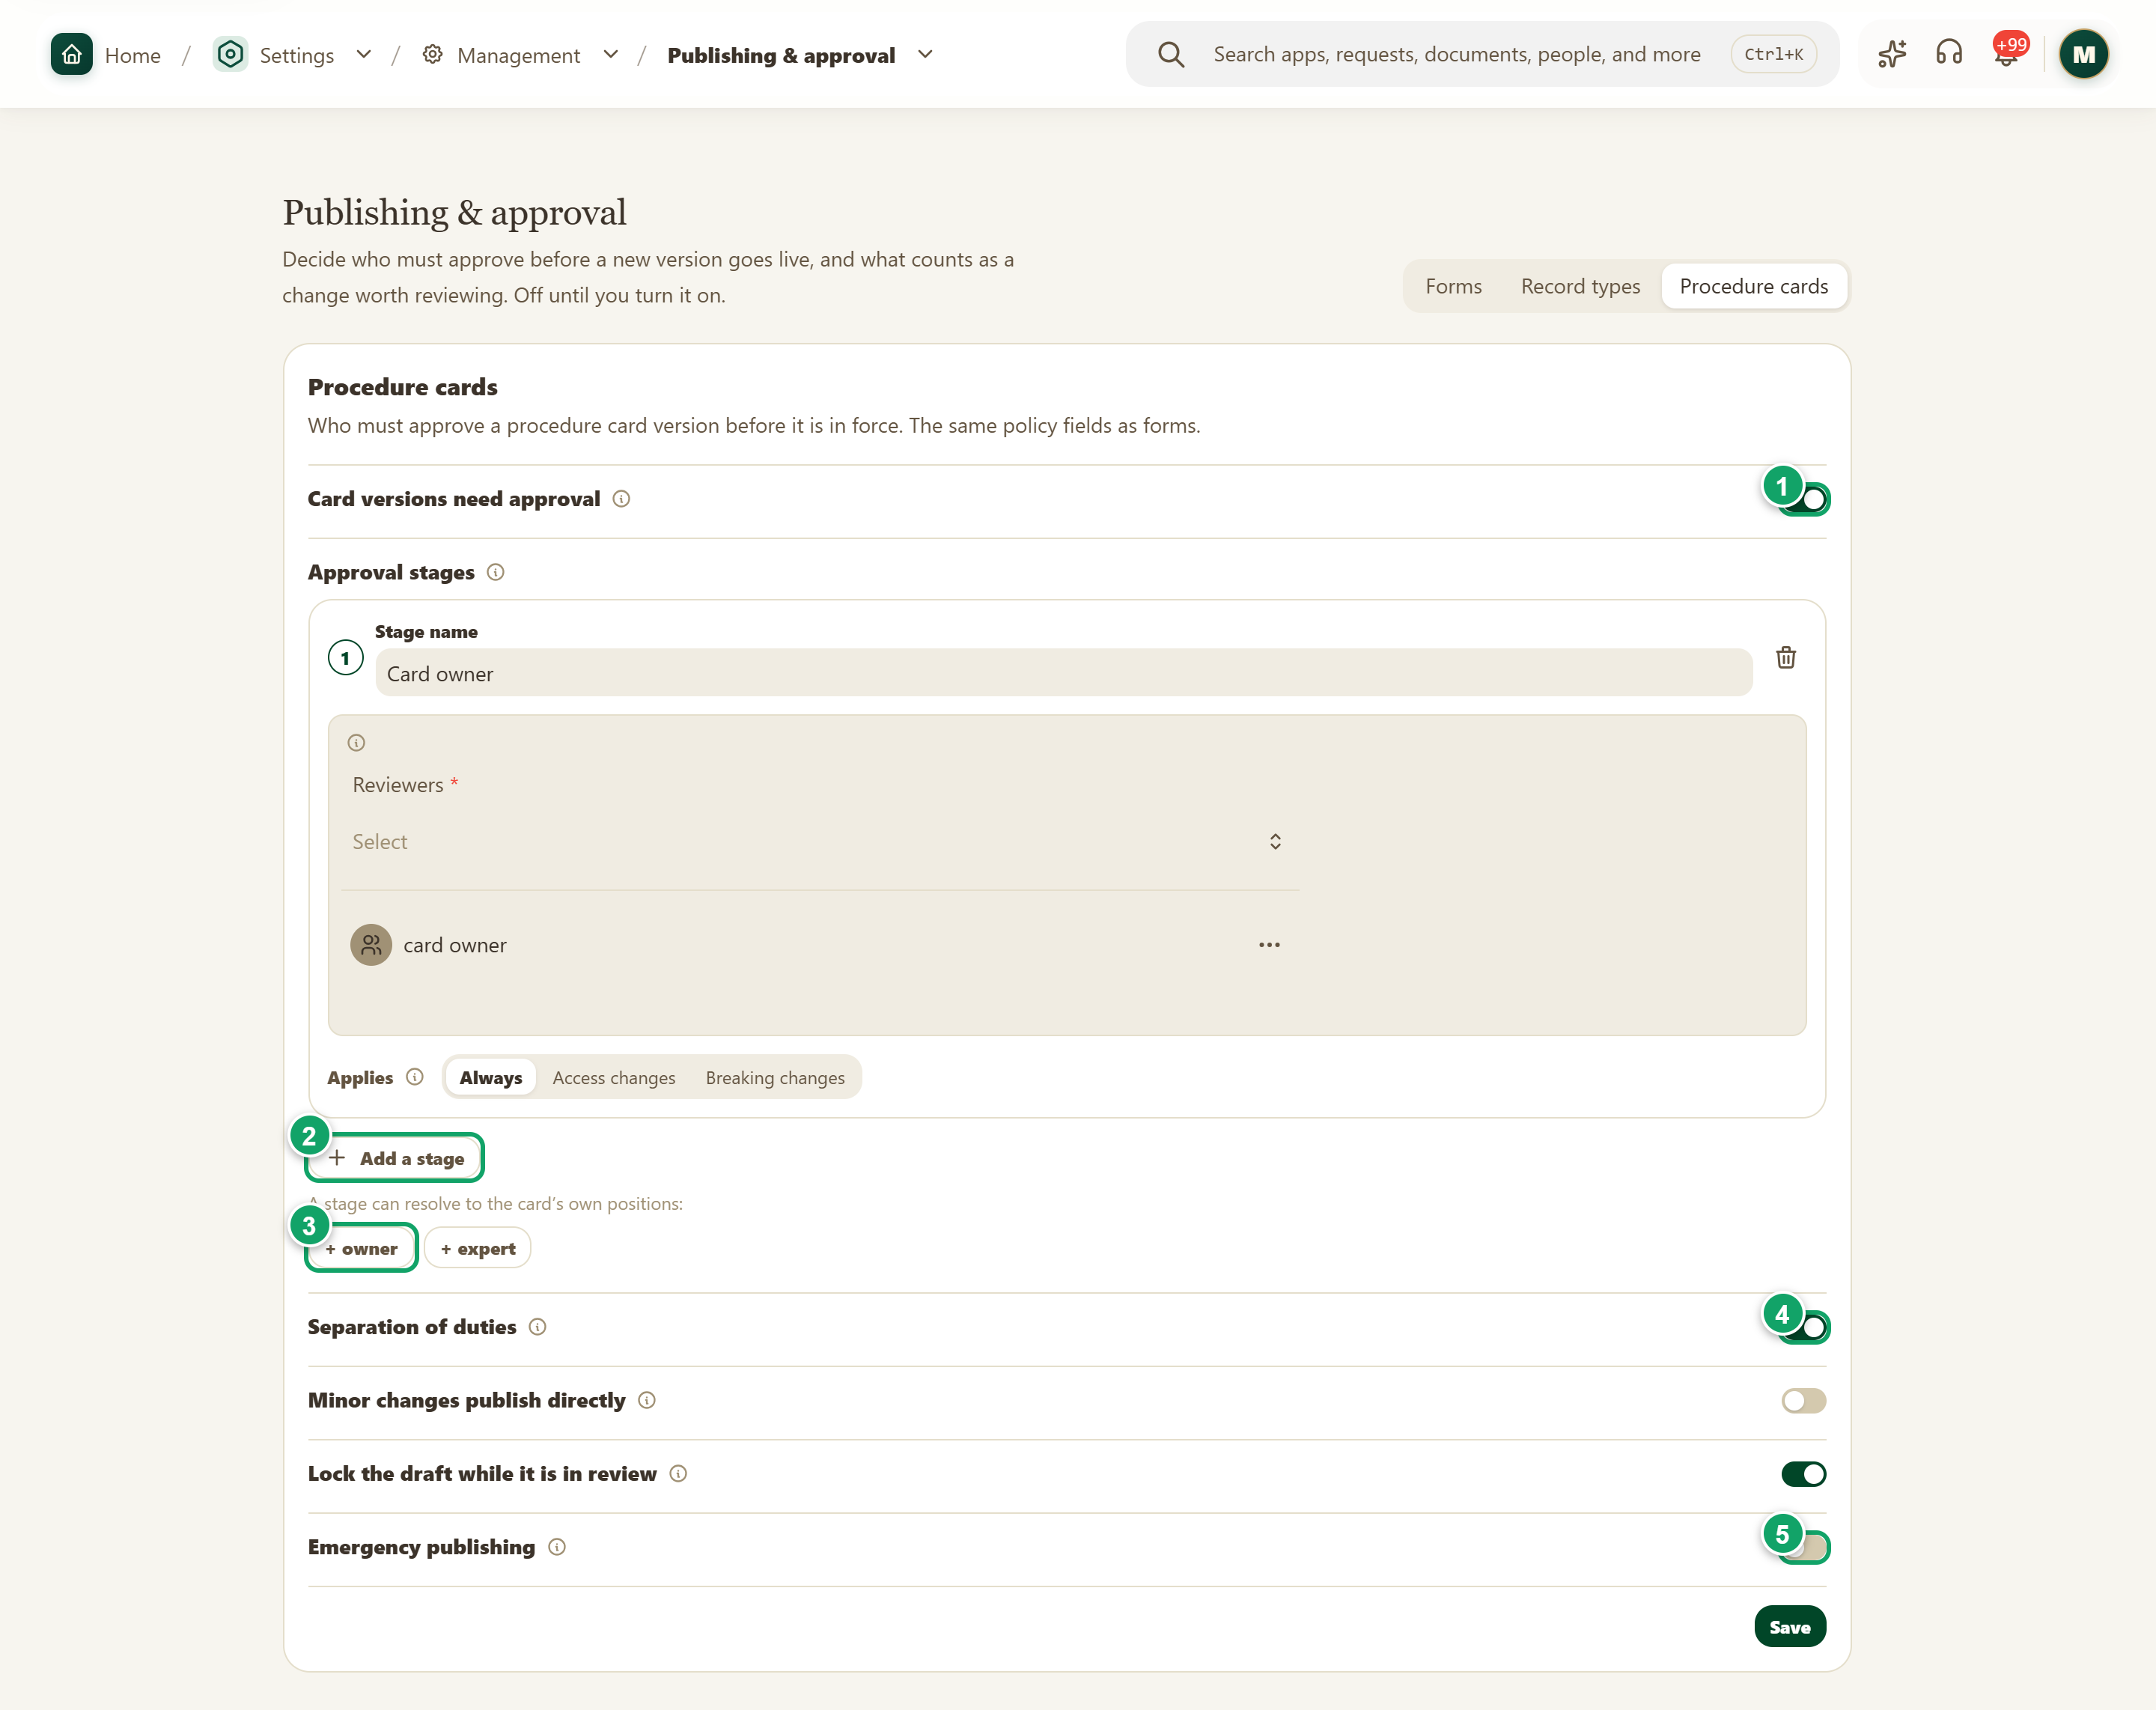
\includegraphics[width=0.95\linewidth,height=0.72\textheight,keepaspectratio]{figures/screens/ch08-publishing-approval-procedure-cards-en.png}
\caption{The policy on the Procedure cards tab}
\label{fig:settings-publishing-approval-procedure-cards-screen}
\shotnote{The image shows a policy that is on in the test organization, with one stage held by the card owner. This tab stops a procedure card version taking effect before approval. The position names on it appear in lowercase English in both languages. ① “Card versions need approval”. ② “Add a stage”. ③ The \en{+ owner} button: adds a stage held by the card owner; \en{+ expert} does the same for the card expert. ④ “Separation of duties”: a draft’s editor cannot approve it. ⑤ “Emergency publishing”.}
\end{figure}

\begin{table}[H]
\centering
\caption{What do you record on the Procedure cards tab?}
\label{tab:settings-publishing-approval-procedure-cards}
\begin{tabularx}{\linewidth}{R{4.2cm} Y}
\rcHeaderRow
\thh{Setting} & \thh{What does it decide?}\\
“Approval stages” & Who approves, in what order, and when each stage applies. A stage can resolve to the card’s own positions.\\
“Minor changes publish directly” & When all changes are minor, such as wording and order, the version publishes without approval.\\
“Lock the draft while it is in review” & When on, the draft cannot be edited; when off, an edit withdraws the request.\\
“Emergency publishing” & The people you set may publish without approval, and a later review is due within the days you set.\\
\end{tabularx}
\end{table}

\begin{enumerate}
\item In “Settings”, open “Publishing \& approval”, then choose the tab.
\item Choose the policy’s scope, or turn on the switch in “Procedure cards”.
\item Add at least one stage, write its name, and set its reviewers and when it applies. In “Record types”, choose the “Reviewers”.
\item Review the rules and emergency publishing, then press “Save” on that tab before moving to another.
\end{enumerate}

\textbf{Check:} A saved message appears, and “Publishing works as before while this is off.” disappears from the “Forms” tab. If the button stays disabled there, read the warning beside it, such as “Every stage needs reviewers.”, and complete what is missing. On the first edit after that, the request should reach reviewers rather than publishing directly.

\clearpage
\section{Form assignments}
\label{sec:settings-feature-form-assignments}

An assignment asks someone to fill in a form by a due date. This page sets what all assignments share: when reminders go out and who is told when one is late, which days count toward due dates, and the usual cap per person. These decisions are therefore not repeated in every plan. The page appears for the organization owner and holders of the Administrator role, who alone can change its values.

\begin{rcnote}[Example: Horizon]
The system administrator turns on “Reminders and escalation” at ②, turns off Friday and Saturday at ③ because the company works Sunday to Thursday, and types 10 at ④. When Sarah Al-Khatib assigns Omar Haddad a form, his time limit counts working days only.
\end{rcnote}

\begin{figure}[H]
\centering
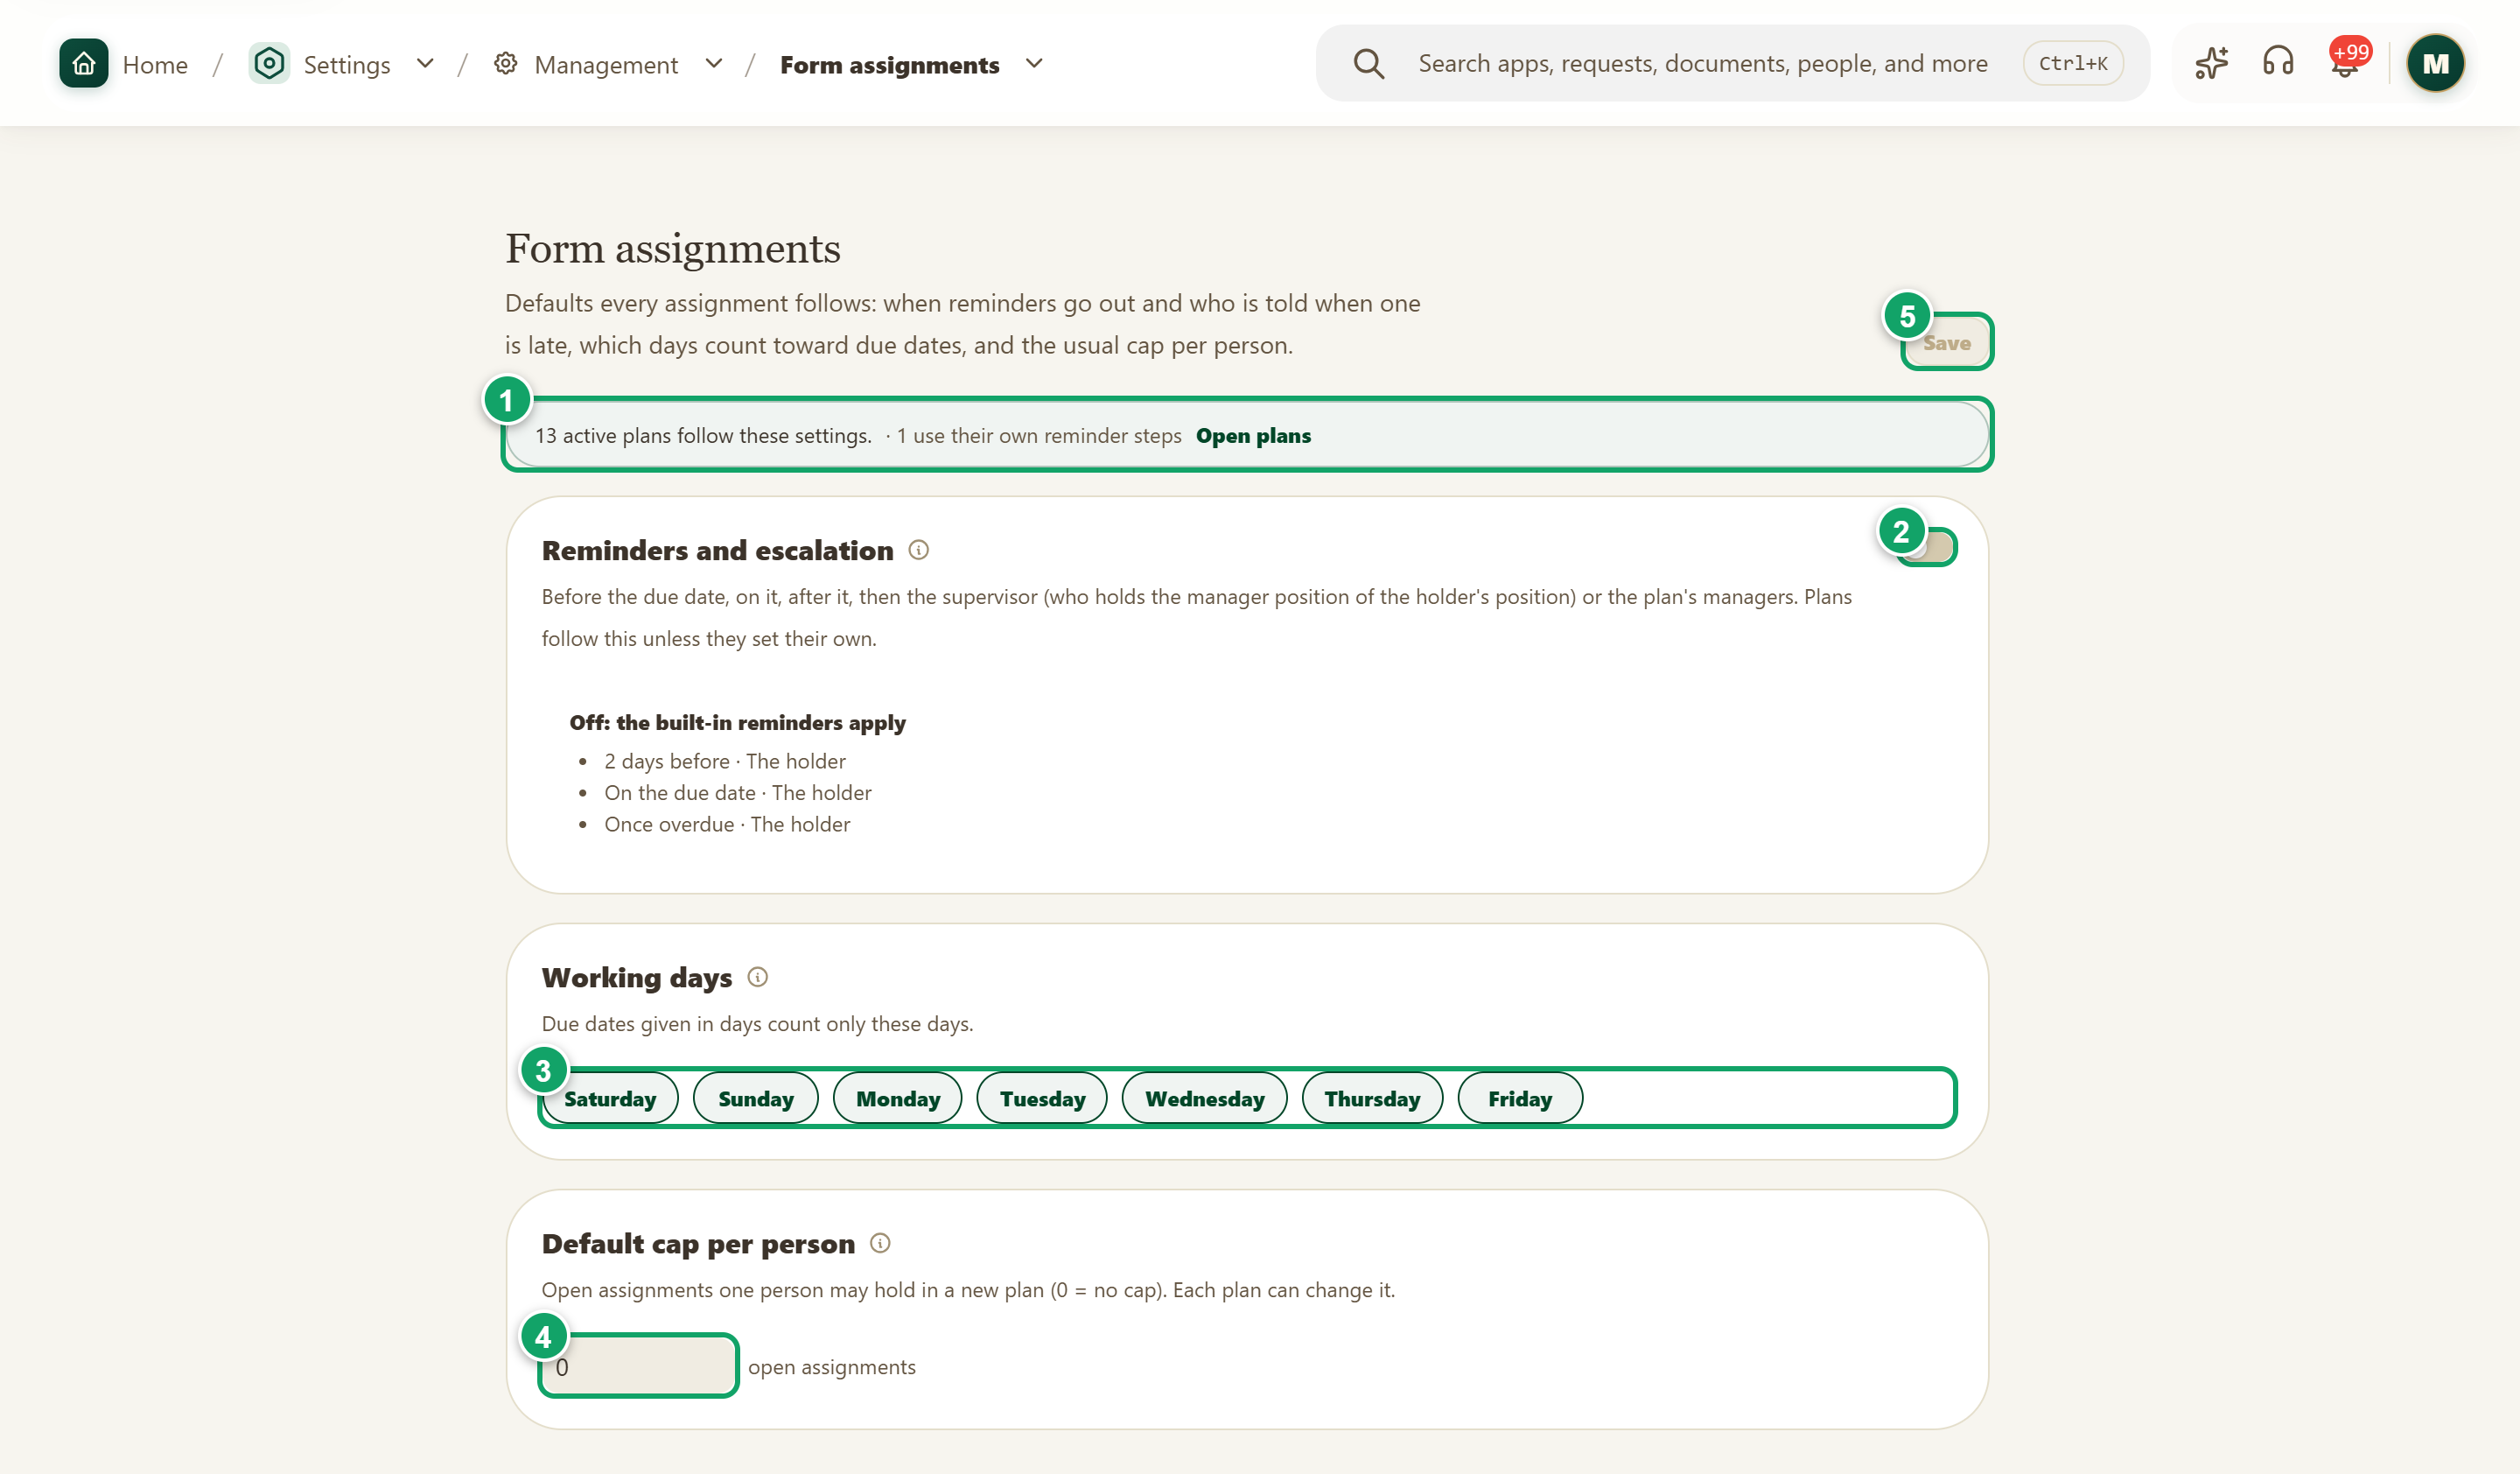
\includegraphics[width=0.95\linewidth,height=0.72\textheight,keepaspectratio]{figures/screens/ch08-form-assignments-en.png}
\caption{The Form assignments page}
\label{fig:settings-form-assignments-screen}
\shotnote{The image shows the test organization’s values: built-in reminders are running, all seven days count, and there is no cap. These are the original values until an organization saves others, so a period in days includes the weekend unless you turn those days off. ① A bar showing how many active plans follow these settings, with “Open plans”. ② The “Reminders and escalation” switch. ③ “Working days”: press a day to turn it off or on; at least one stays on. ④ “Default cap per person”. ⑤ “Save”.}
\end{figure}

\begin{figure}[H]
\centering
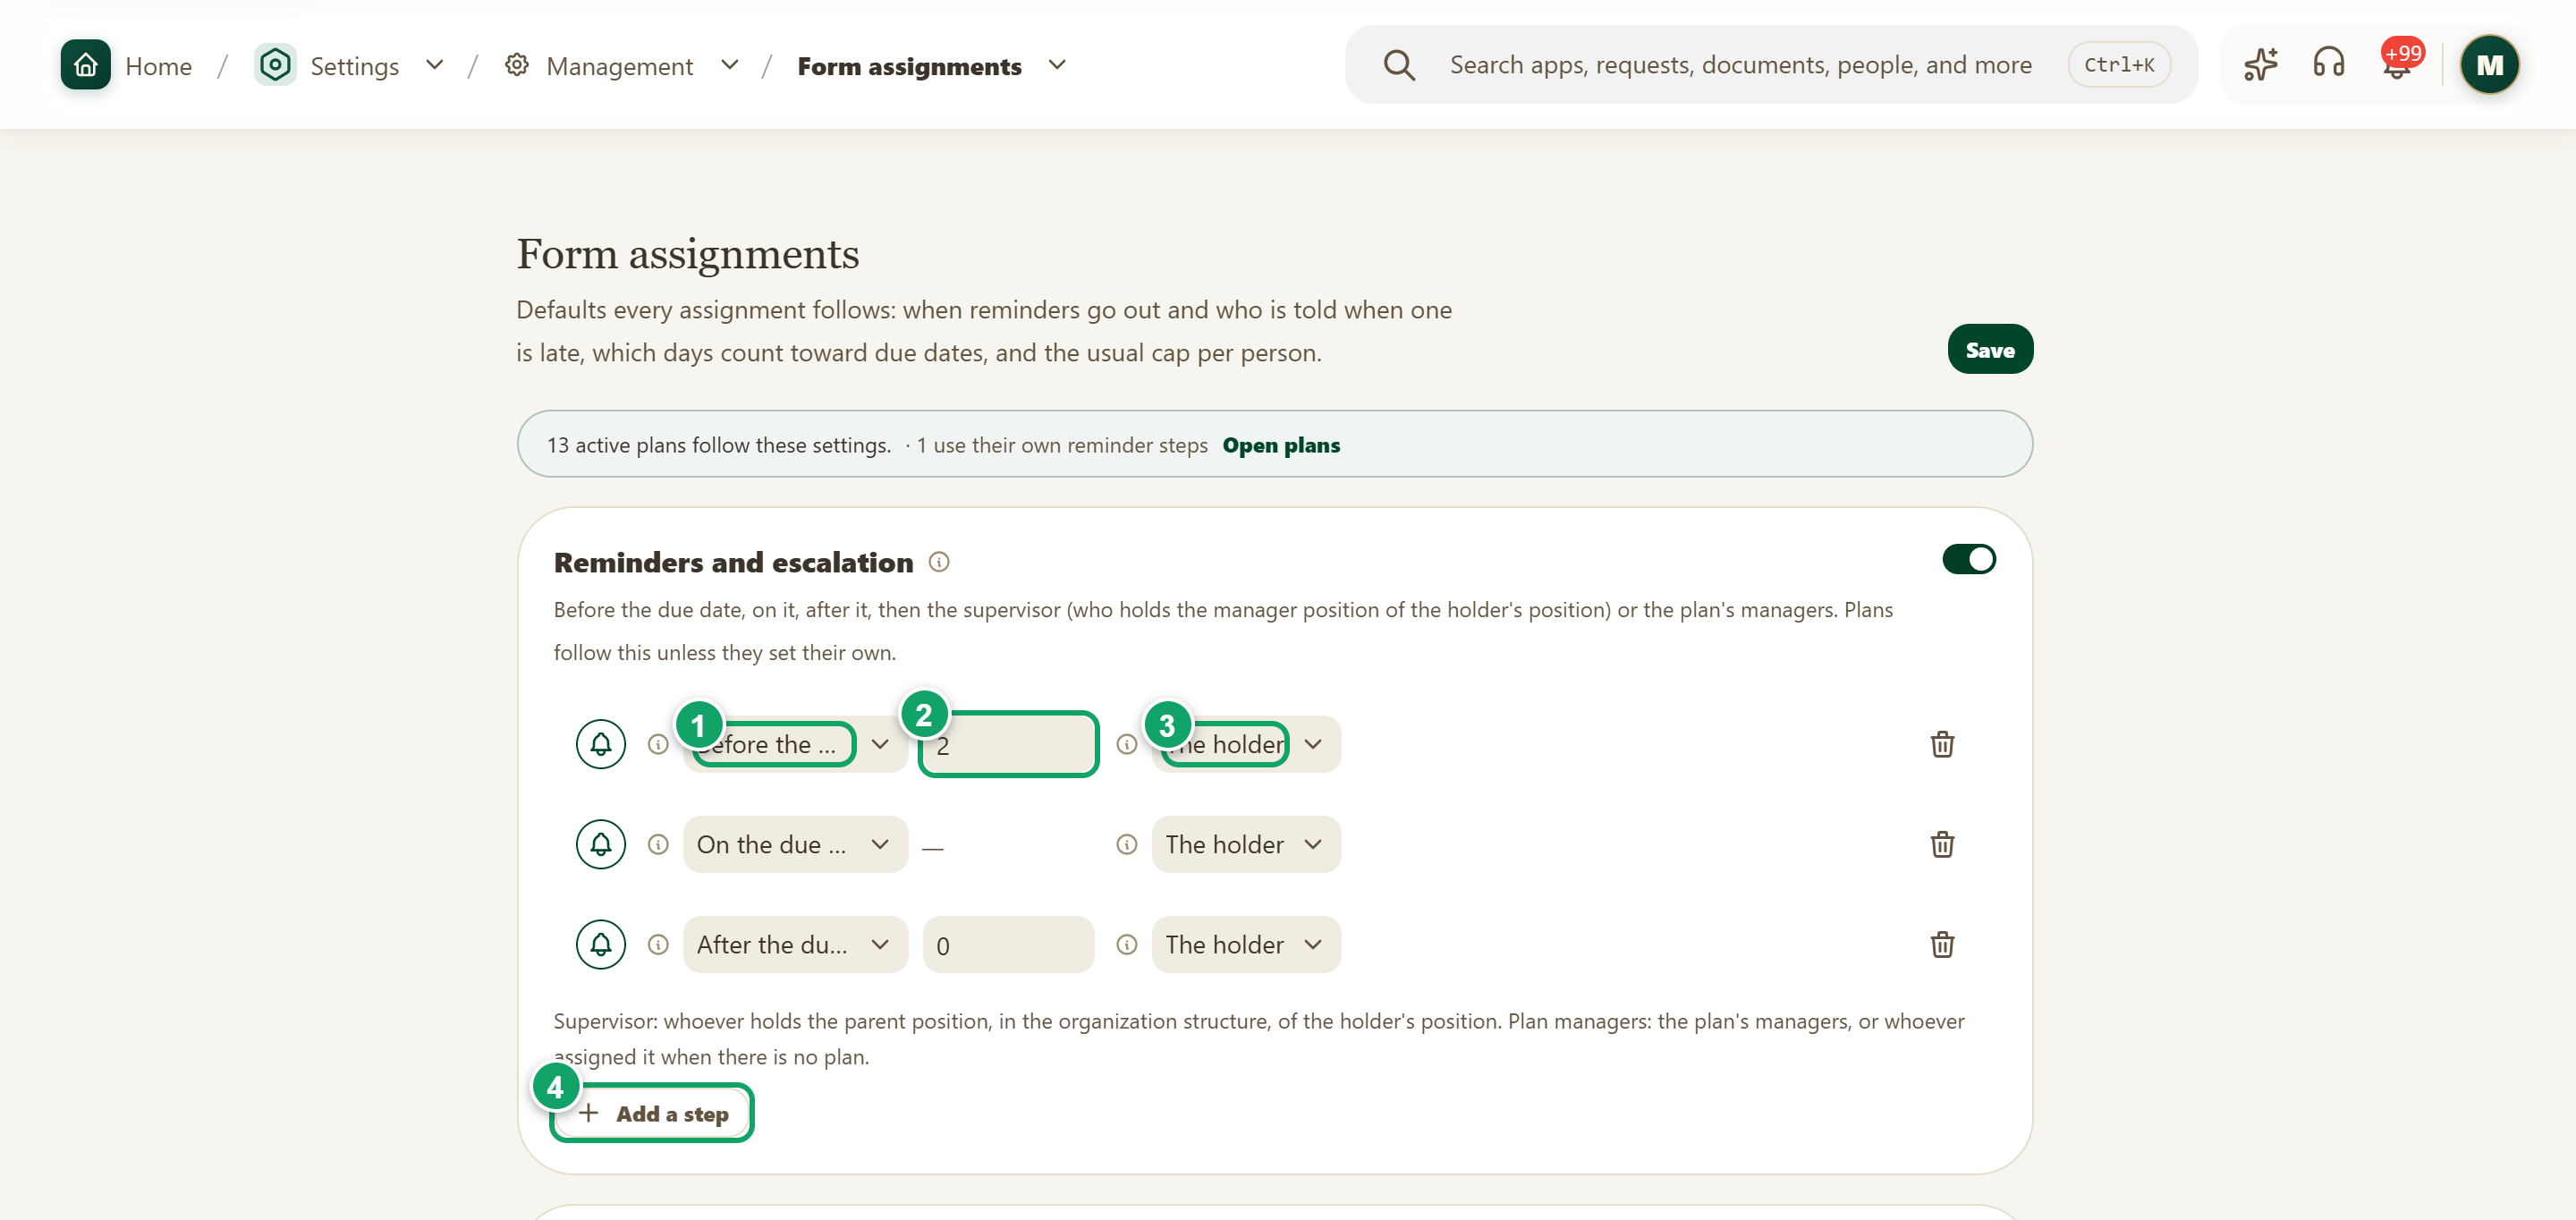
\includegraphics[width=0.95\linewidth,height=0.72\textheight,keepaspectratio]{figures/screens/ch08-form-assignments-ladder-en.png}
\caption{Reminder steps with the switch on}
\label{fig:settings-form-assignments-ladder-screen}
\shotnote{The image shows the switch on without saving; the steps start as a copy of the built-in reminders, so you edit them rather than start from nothing. Each row is a step that answers two questions: when the reminder goes, and to whom. ① When: “Before the due date”, “On the due date” or “After the due date”. ② The number of days, up to 60. ③ To whom: “The holder”, “Their supervisor”, “Plan managers” or “By code”. ④ “Add a step”: up to 8 steps.}
\end{figure}

\begin{table}[H]
\centering
\caption{What do you record in Form assignments?}
\label{tab:settings-form-assignments-fields}
\begin{tabularx}{\linewidth}{R{4.2cm} Y}
\rcHeaderRow
\thh{Setting} & \thh{What do you record?}\\
“Reminders and escalation” & When off, the built-in reminders go to the holder: 2 days before, on the due date and once overdue. When on, your steps apply. Plans follow them unless they set their own.\\
“Their supervisor” & Whoever holds the parent position of the holder’s position in the organization structure.\\
“Plan managers” & The plan’s managers, or whoever assigned it when there is no plan.\\
“By code” & An expression that works out the recipients; it needs someone who can write expressions. Use the other three options when they are enough.\\
“Working days” & The days that count in due dates given in days.\\
“Default cap per person” & Open assignments one person may hold in a new plan, from 0 to 500, where 0 means no cap. Each plan can change it.\\
\end{tabularx}
\end{table}

\begin{enumerate}
\item In “Settings”, open “Form assignments”, and read the bar to see how many plans are affected.
\item Turn on “Reminders and escalation”, then edit the steps or add a step after the due date to “Their supervisor”.
\item Set the “Working days”, then type the “Default cap per person”.
\item Press “Save”.
\end{enumerate}

\textbf{Check:} “Saved.” appears and the values remain when you reopen the page. A plan with its own steps keeps them, and the bar shows how many do. The new cap starts with new plans.

\clearpage
\section{Check categories}
\label{sec:settings-feature-check-categories}

A check is a rule in a form that alerts a reviewer to a value that needs a look. This page sets the categories checks are filed under, such as consistency or capacity, so reviewers and dashboards can group them. You need it when checks multiply and become hard to follow. Any member can read the categories; only the organization owner and holders of the Administrator role can change them.

\begin{rcnote}[Example: Horizon]
The system administrator presses “Add category” at ④, writes “Branch data” at ①, chooses its color at ②, then presses “Save” at ⑤. Sarah Al-Khatib can then choose this category for a check in the visit request form.
\end{rcnote}

\begin{figure}[H]
\centering
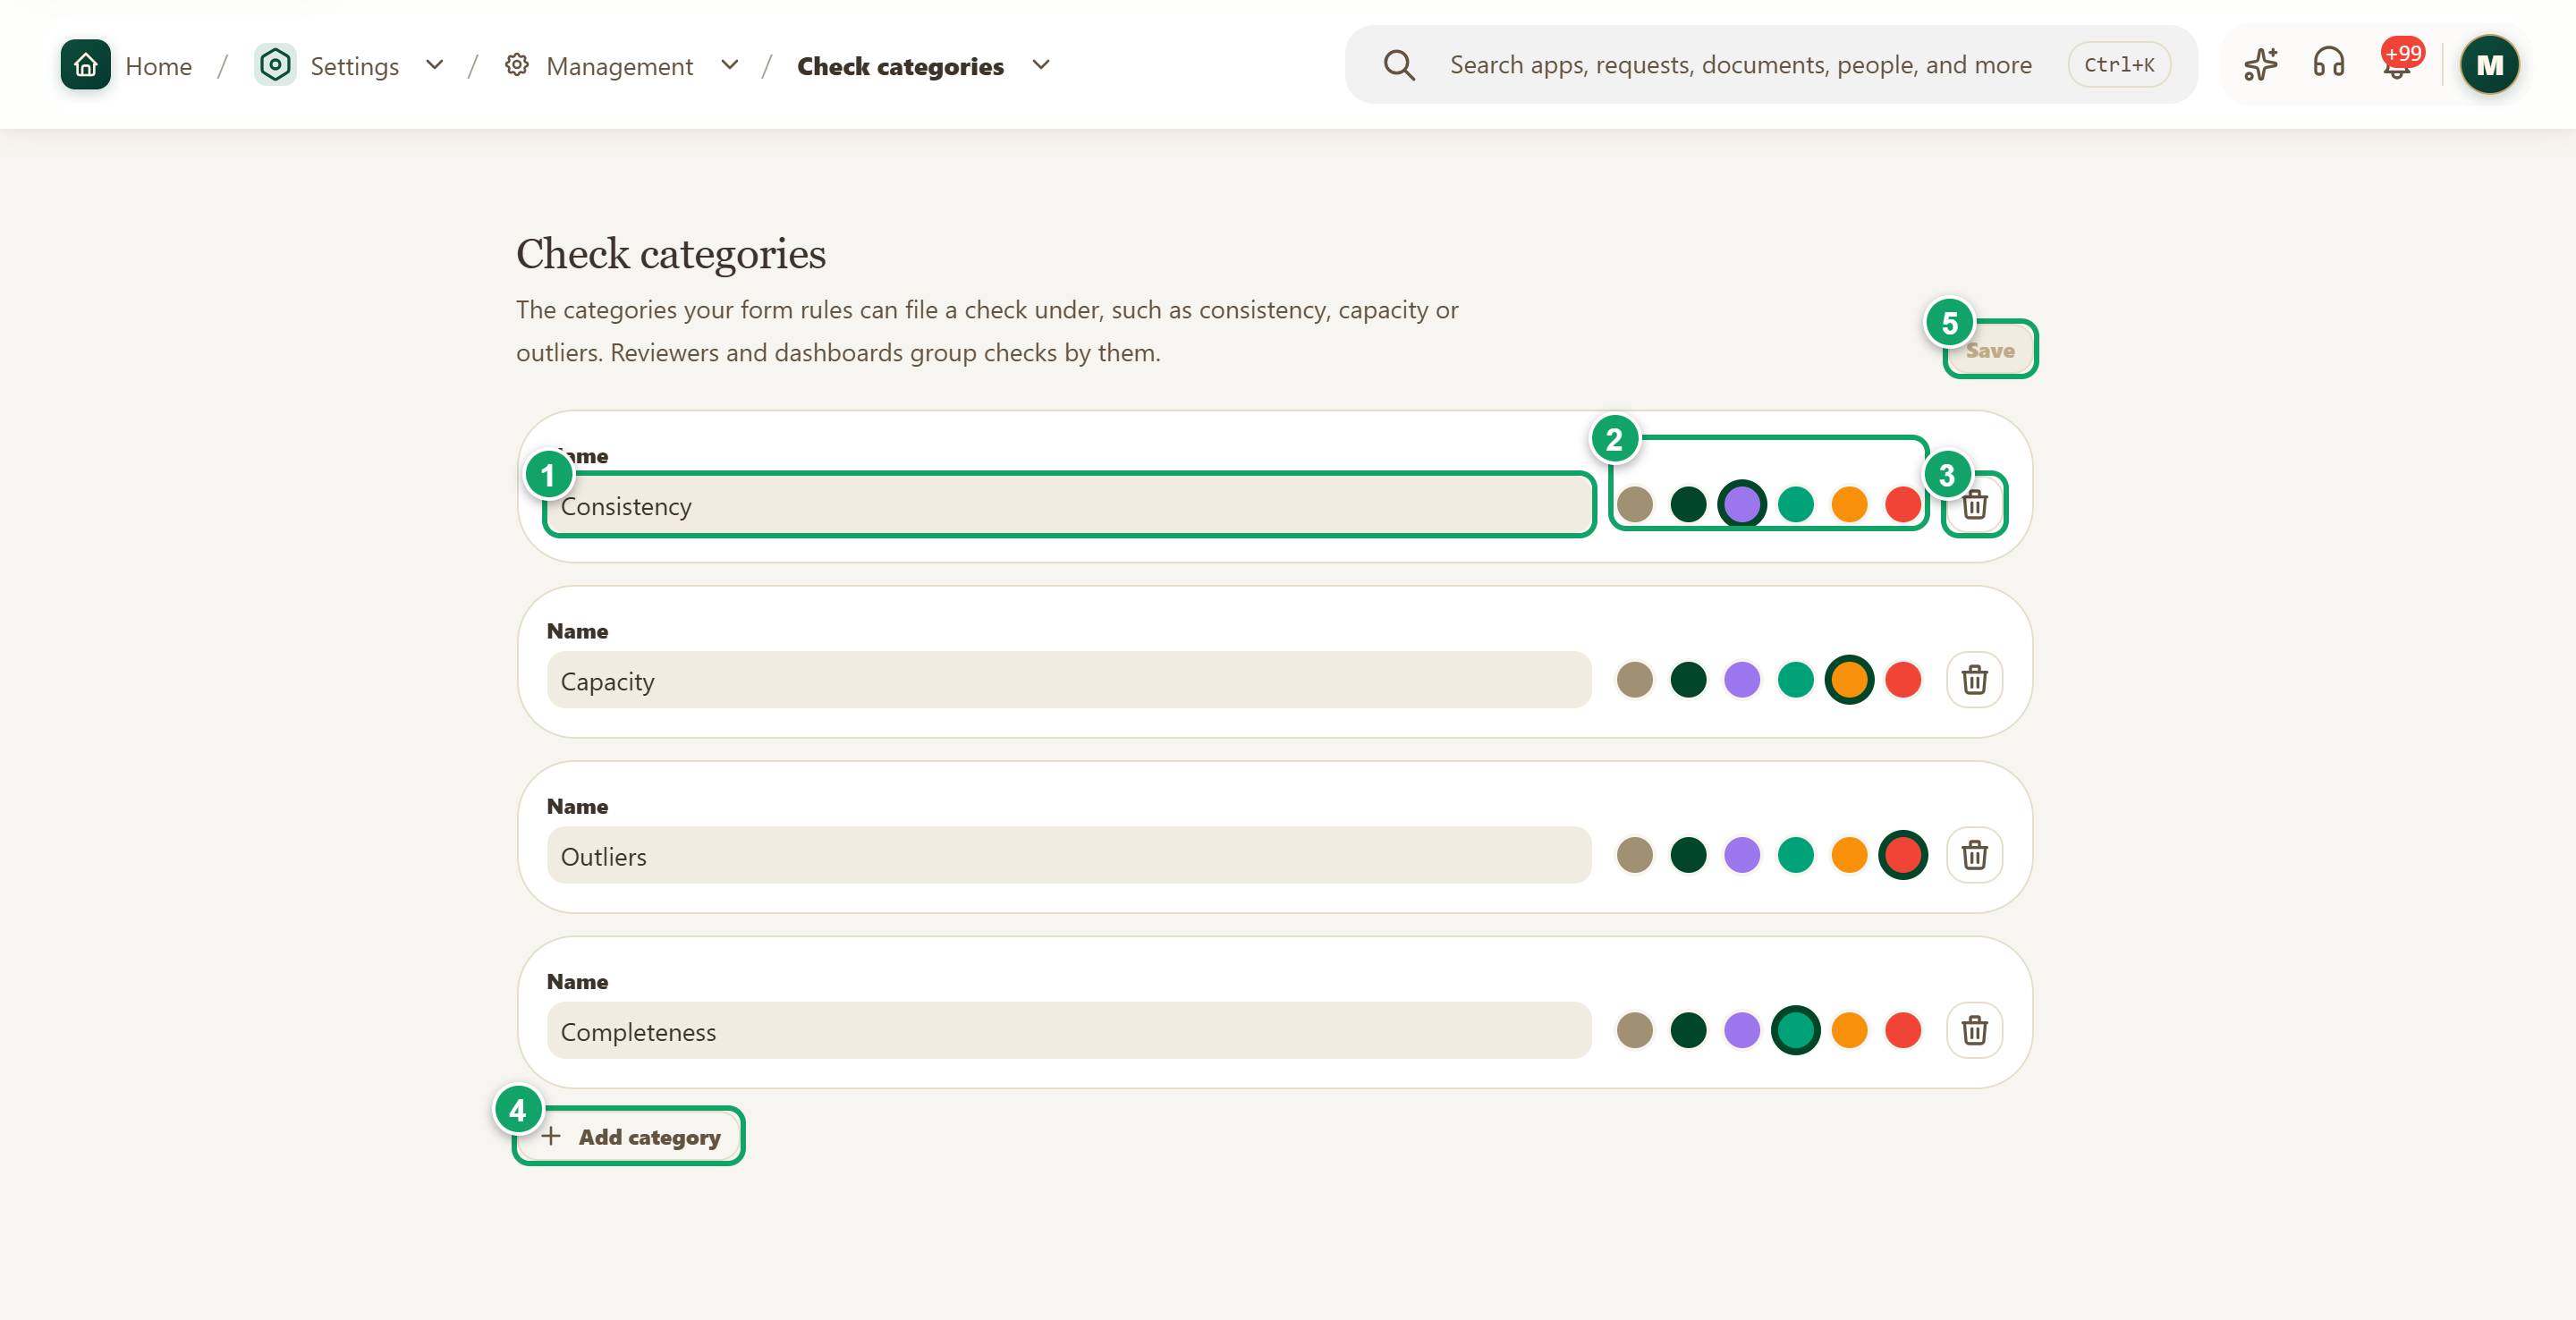
\includegraphics[width=0.95\linewidth,height=0.72\textheight,keepaspectratio]{figures/screens/ch08-check-categories-en.png}
\caption{The list of check categories}
\label{fig:settings-check-categories-screen}
\shotnote{The image shows the four categories in the test organization; nothing changed here applies until you press “Save”. Each card is a category form rules can choose, and renaming it keeps the checks linked to it grouped under it. ① “Name”: up to 80 characters, written per language with the language buttons. ② “Colour”: six colors. ③ “Remove category”: the row disappears with no confirmation, and removal is complete only after saving. ④ “Add category”. ⑤ “Save”: stays disabled until something changes, and while a category has no name.}
\end{figure}

\begin{table}[H]
\centering
\caption{What do you record in a check category?}
\label{tab:settings-check-categories-fields}
\begin{tabularx}{\linewidth}{R{4.2cm} Y}
\rcHeaderRow
\thh{Field} & \thh{What do you record?}\\
“Name” & The category’s name as the reviewer sees it, in at least one language. You can add up to 50 categories.\\
“Colour” & A color that helps tell the category apart. A new category gets a starting color you can change.\\
\end{tabularx}
\end{table}

\begin{enumerate}
\item In “Settings”, open “Check categories”, then press “Add category”.
\item Write the “Name” and choose the “Colour”.
\item Press “Save”.
\item In the form’s rules, open the check and pick the category in the “Category” field.
\end{enumerate}

\textbf{Check:} “Saved.” appears and the category stays in the list after you reopen the page. If you delete a category a rule uses, the rule keeps it until you change it and shows its internal value, so update the rules before deleting.
